\documentclass[a4paper, 12pt]{article}
\usepackage[utf8]{inputenc}
\renewcommand\familydefault{\sfdefault}
\usepackage[T1]{fontenc}
\usepackage[francais]{babel}
\usepackage[left=2.5cm,top=2.5cm,right=2.5cm,bottom=2.5cm]{geometry}
\usepackage[onehalfspacing]{setspace}
\usepackage{graphicx}
\usepackage[usenames, dvipsnames]{xcolor}
\definecolor{mygray}{gray}{0.95}

\usepackage{minted}
\usemintedstyle{colorful}
\usepackage{float}
\floatplacement{figure}{H}
\usepackage{authblk}
\usepackage{enumitem}
\setlist[enumerate]{label*=\arabic*.}
\usepackage{hyperref}
\hypersetup{
    colorlinks,
    citecolor=black,
    filecolor=black,
    linkcolor=black,
    urlcolor=blue
}

\usepackage{caption}
\newenvironment{code}{\captionsetup{type=listing}}{}
\usepackage{array}
\usepackage{etoolbox}
\patchcmd{\thebibliography}{\section*{\refname}}{}{}{}

\usepackage{dirtree}
\usepackage{tabularx}

\usepackage{glossaries}
	\let\oldnewacronym\newacronym
	\newcommand*{\provideacronym}[3]{%
	  \ifglsentryexists{#1}{%
	  }{%
	    \oldnewacronym{#1}{#2}{#3}%
	  }%
	}
\makeglossaries

\usepackage{fancyhdr}
\pagestyle{fancy}
\fancyhf{}
\lhead{Projet IoT}
\rhead{\leftmark}
\lfoot{Jeremy Favre - Steven Liatti}
\rfoot{\thepage}
\renewcommand{\footrulewidth}{1pt}

\usepackage{pdfpages}

\begin{document}

\title{Projet IoT}
\author{Jeremy Favre - Steven Liatti}
\date{Janvier 2020}
\maketitle
% \begin{figure}
%     \begin{center}
%         \includegraphics[width=0.65\textwidth]{img/screenshots/movie_list_framed.png}
%     \end{center}
% \end{figure}
\newpage


% \setcounter{tocdepth}{2}
\addcontentsline{toc}{subsection}{Table des matières}
\tableofcontents
\addcontentsline{toc}{subsection}{Table des figures}
\listoffigures
% \renewcommand{\listtablename}{Table des tables}
% \addcontentsline{toc}{subsection}{Table des tables}
% \listoftables
\newpage
\renewcommand\listoflistingscaption{Table des listings de code source}
\addcontentsline{toc}{subsection}{Table des listings de code source}
\listoflistings

\subsection*{Conventions typographiques} %-----------------------------------------------------------------------------------------------
\addcontentsline{toc}{subsection}{Conventions typographiques}
Lors de la rédaction de ce document, les conventions typographiques ci-dessous ont
été adoptées.
\begin{itemize}[label=\textbullet]
	\item Tous les mots empruntés à la langue anglaise ou latine ont été écrits en \textit{italique}.
	\item Toute référence à un nom de fichier (ou répertoire), un chemin d'accès, une 
    utilisation de paramètre, variable, commande utilisable par l'utilisateur, ou extrait de code 
    source est écrite avec une police d'écriture à \mintinline{text}{chasse fixe}.
	\item Tout extrait de fichier ou de code est écrit selon le format suivant:
    \bigbreak
    \begin{code}
        \begin{minted}[bgcolor=mygray,breaklines,breaksymbol=,linenos,frame=single,stepnumber=1,tabsize=2]{kotlin}
fun main() {
    println("Hello World!")
}
        \end{minted}
    \end{code}
\end{itemize}


\newacronym{api}{API}{\textit{Application Programming Interface}, Interface de programmation : services offerts par un programme producteur à d'autres programmes consommateurs}
\newacronym{json}{JSON}{\textit{JavaScript Object Notation}, Format d'échange de données léger, facile à lire et écrire par les humains et les machines}
% \newacronym{xml}{XML}{\textit{Extensible Markup Language}, Langage extensible de description de données}
% \newacronym{jvm}{JVM}{\textit{Java Virtual Machine}, Exécute le bytecode Java sur différents systèmes d'exploitation}
\printglossary[type=\acronymtype,title={Acronymes}]
\newpage


\section{Introduction} %-----------------------------------------------------------------------------------------------
Ce projet concerne le dévelopement d'un logiciel de construction moderne qui offre des fonctionnalités de haut niveau (fonctionnalités pour l'utilisateur final) telles que :
\begin{itemize}
    \item Abaisser la température d'une pièce à un seuil donné lorsqu'elle est vide
    \item Augmenter la température d'une pièce à un seuil donné lorsqu'elle est occupée
    \item Fermer les stores lorsque l'humidité est élevée
    \item Ouvrir les stores le jour, lorsque la luminance est faible et que la pièce est occupée
    \item Afficher l'état d'un magasin et / ou d'un radiateur donné
    \item Surveiller manuellement les stores et les radiateurs de la pièce où se trouve l'utilisateur
    \item Fournir des statistiques
\end{itemize}
Ces fonctionnalités peuvent être activées automatiquement ou manuellement. La forme "nous" est utilisée tout au long de ce rapport étant donné que ce projet est réalisé par binôme.

\subsection{Buts}
Le but de cette application est de mettre en pratique les différentes librairies et tecchnologies étudiées en cours d'internet des objets afin de produire une interafce utilisateur déployée sur un smartphone Android.

\subsection{Motivations}
Le périmètre de ce projet semblait parfaitement adapté pour exploiter la majorité des techniques et méthodes vues durant le cours d'IOT. Ce projet est une formidable occasion pour relier la mise en pratique des connaissances acquises en cours et notre passion pour le dévloppement full stack.

\subsection{Méthodologie de travail}
Sur la base d'une analyse préliminaire, nous avons séparé le travail en plusieurs tâches que nous avons assigné à chaque membre du binôme de manière équitable afin d'effectuer le travail en parallèle.
Nous avons adopté une pseudo méthode "agile", en factorisant le projet en petites tâches distinctes et en nous fixant des délais pour les réaliser. Le partage du code s'est fait avec git et gitlab. Nous nous sommes servis des \textit{issues} gitlab pour représenter nos tâches et du "board" du projet pour avoir une vision globale du travail accompli (par qui et quand) et du travail restant.

% TODO: remove
\cite{tmdb} \cite{book}
\newpage

\section{Conception et analyse} %-----------------------------------------------------------------------------------------------
\begin{figure}
    \begin{center}
        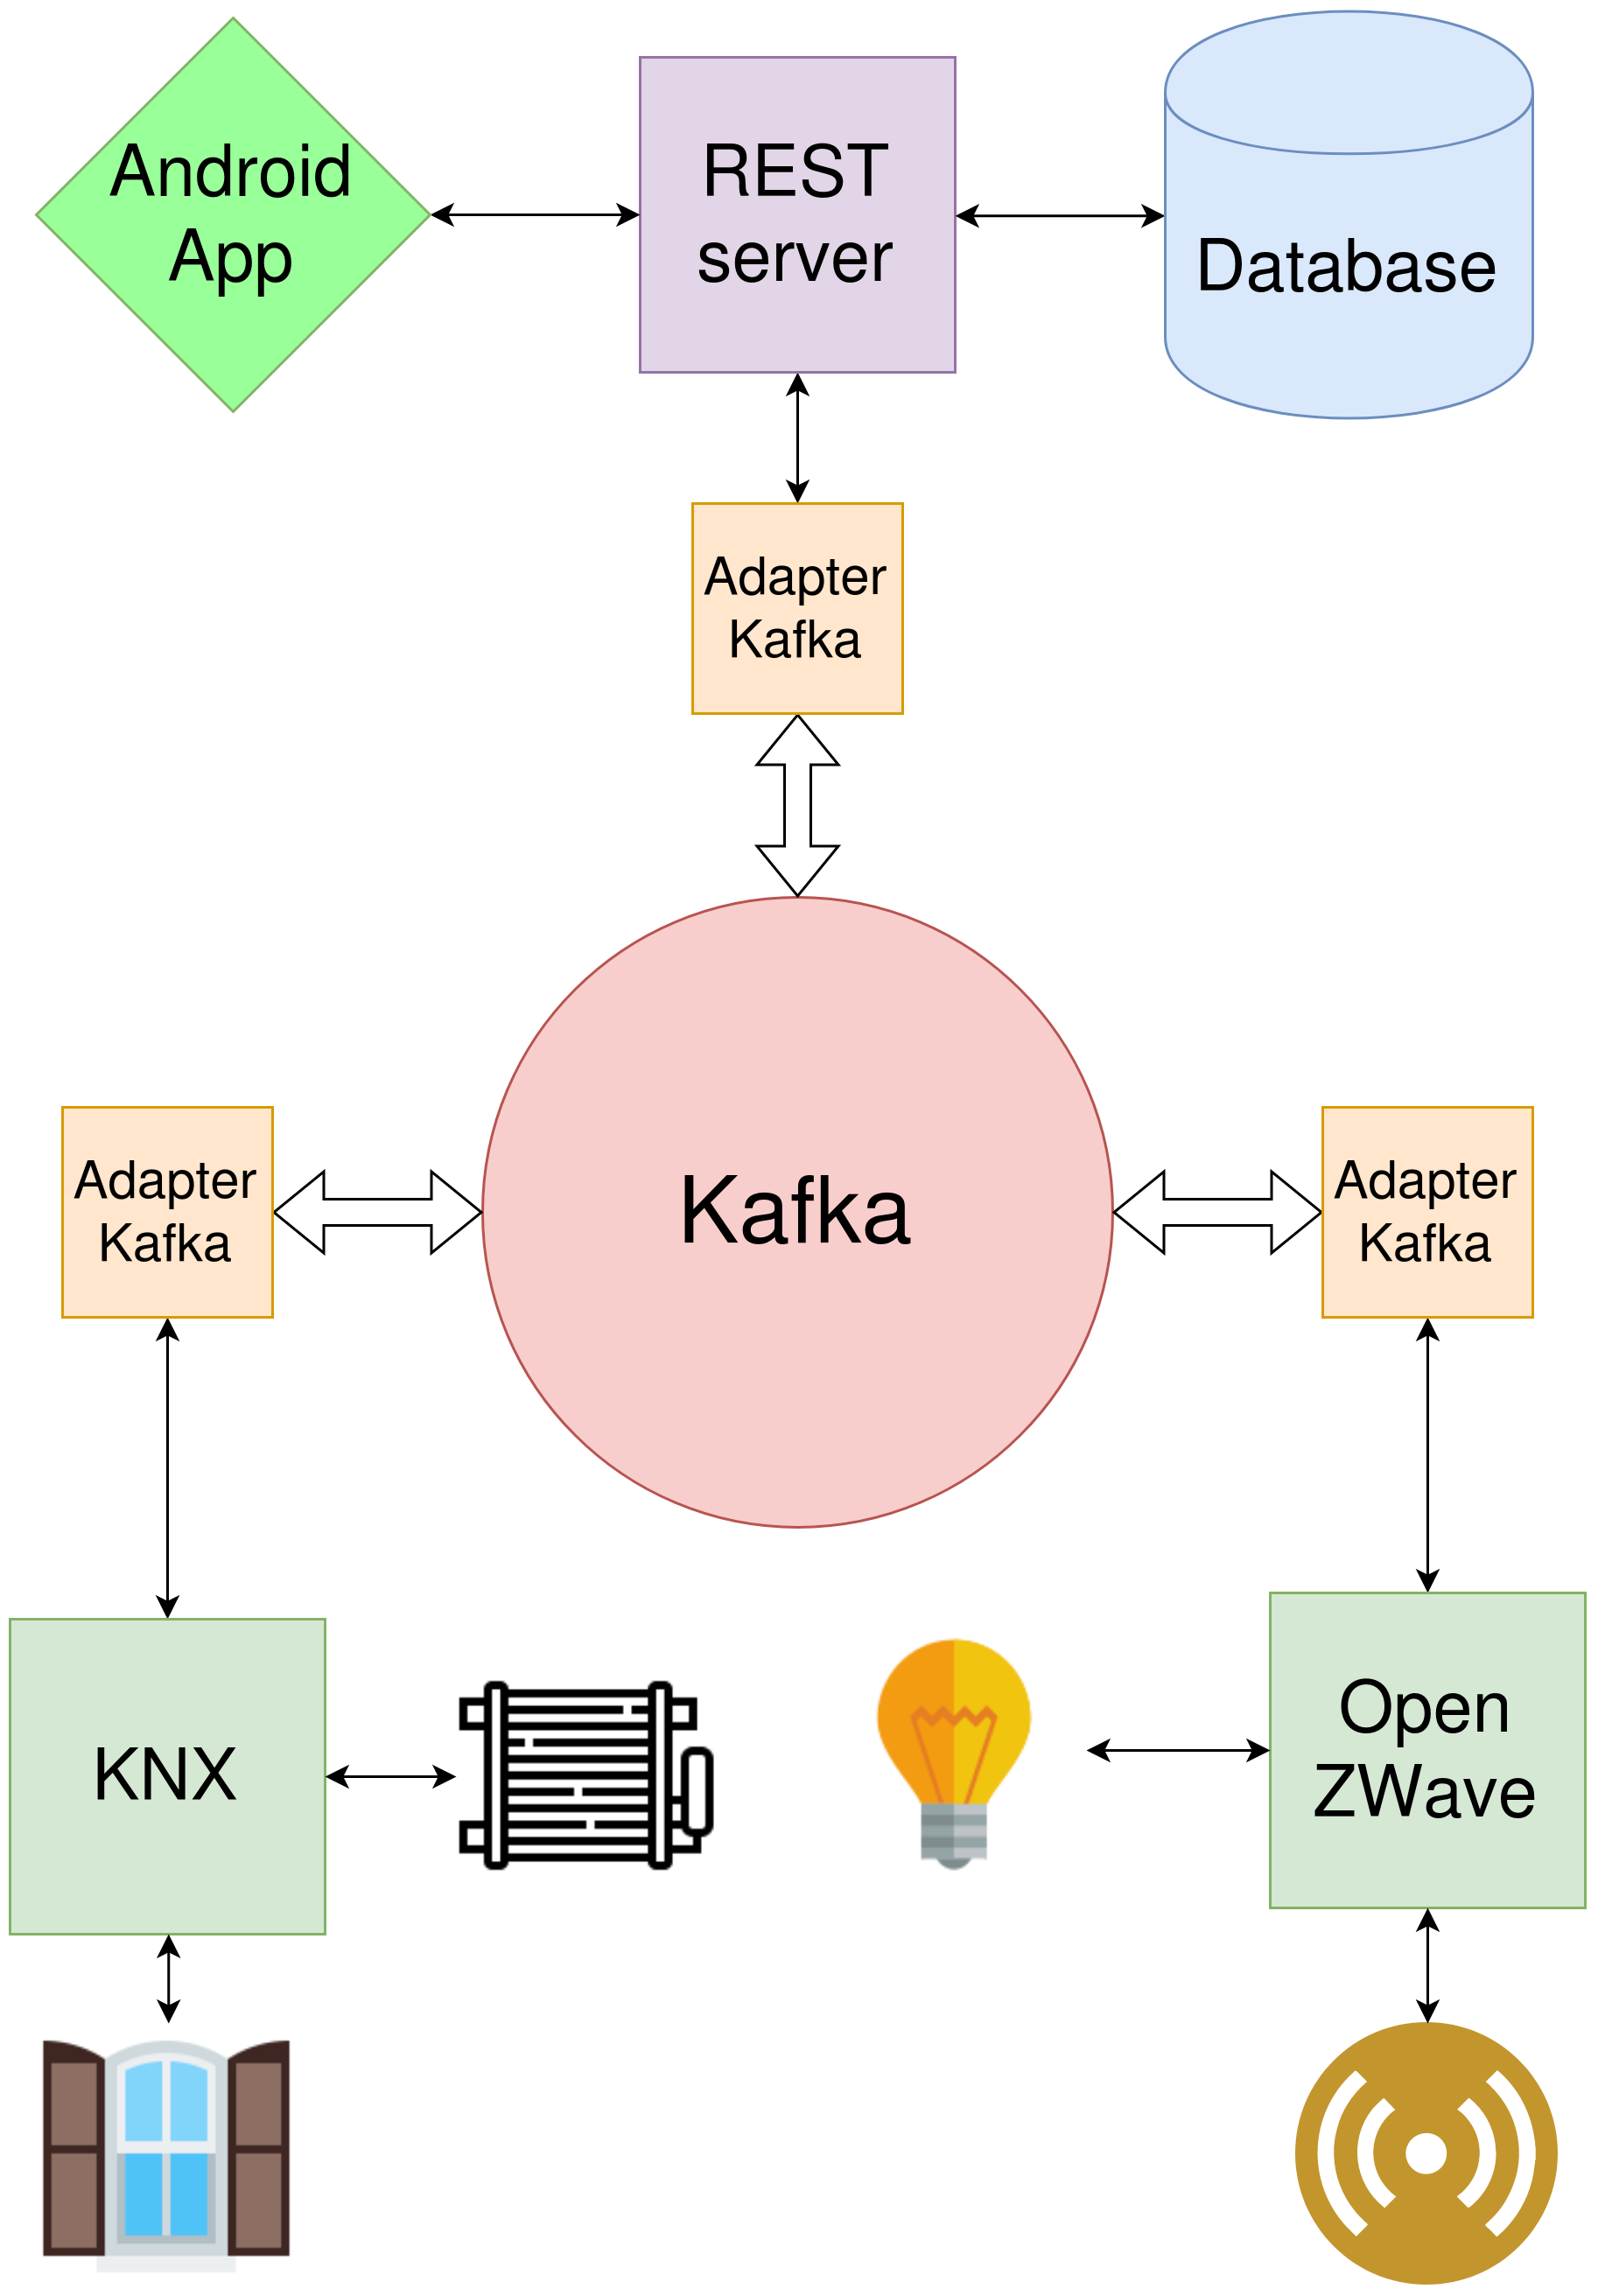
\includegraphics[width=0.8\textwidth]{img/general.png}
    \end{center}
    \caption{Architecture globale du système}
    \label{shema_general}
\end{figure}


\subsection{Protocole d'échange des messages}
Le Protocole d'échange des messages à été défini selon l'arcitecture visible à la figure "Architecture globale du système", les entités principales de l'application sont le client mobile, les devices KNS, les devices Openzwave et la base de données. Afin de tout mettre le tout en relation, nous avons procédé de manière à échanger les messages dans différents "topics" qui permettent d'identifier le sujet des messages.

\subsection{Statistiques}
En ce qui concernet les Statistiques, notre architecture de la base de données est pensée de manière à stocker les informations des différents devices dans le temps afin de pouvoir retraçer leurs parcours et établir les statistiques qui en découlent.
\newpage

\section{Kafka} %-----------------------------------------------------------------------------------------------
\subsection{Kafka}
La technologie d'échange des messages était au choix, nous avons choisi d'experimenter kafka étant donné qu'elle est de plus en plus répendue dans les différents projets, il était donc interessant de la prendre en main au travers de ce projet.
\subsubsection{Généralités}
Apache Kafka est une plate-forme de diffusion d'événements distribuée open source, tolérante aux pannes, développée par LinkedIn. Service de journalisation distribué, Kafka est souvent utilisé à la place des courtiers de messages traditionnels en raison de son débit, de son évolutivité, de sa fiabilité et de sa réplication plus élevés. Étant donné que Kafka est un système distribué, les rubriques sont partitionnées et répliquées sur plusieurs noeuds.

Elle permet principalement de :
\begin{itemize}
    \item Publier et s'abonner à des flux d'enregistrements, similaires à une file d'attente de messages ou à un système de messagerie d'entreprise.
    \item Stocker les flux d'enregistrements d'une manière durable à tolérance de pannes
    \item Traiter les flux d'enregistrements au fur et à mesure qu'ils se produisent.
\end{itemize}

Les API kafka suivantes sont utilisées dans ce projet :
\begin{itemize}
    \item L'API Producer permet à une application de publier un flux d'enregistrements sur un ou plusieurs sujets Kafka.
    \item L'API Consumer permet à une application de s'abonner à un ou plusieurs sujets et de traiter le flux d'enregistrements qui leur est produit.
\end{itemize}

\subsubsection{Usage dans le projet}
Dans le cadre de ce projet, nous avons utilisé kafka afin de communiquer entre les différentes entités de l'application.
Chacunes d'entre elles (knx, openzawe, API rest Flask) écoute et produit différents messages dans kafka afin de réagire à certains actions et également de produire des informations sans dépendre de la demande demande des client. Au sein de ce projet, nous faisons usage de deux topics principaux "KNX" et "Zwave" qui nous permettent aux différents services d'éméttre et récéptionner les messages qui les concrenent.

\newpage

\section{Implémentation} %-----------------------------------------------------------------------------------------------
\subsection{Application client}
Le client developpé est une application Android. Nous avons choisi d'utiliser le langage Kotlin qui est plus performant et optimise les opérations et la structure par rapport à Java. C'est également le langage que nous utilisons au sein du cours d'Android, c'est donc un bon moyen de mettre en relation les deux cours.
Le rôle principal de ce client est de détecter (grâce au bluetooth) le Beacon le plus proche. En fonction de ce Beacon, le serveur Flask \acrshort{rest} est interrogé pour déterminer (via la base de données) dans quelle salle se trouve la personne et les \textit{\textit{devices}} présents (stores, radiateurs, lumières, etc.). Une fois l'emplacement déterminé et les \textit{\textit{devices}} détectés, les contrôles et les informations des différents \textit{\textit{devices}} apparaissent sur l'interface graphique de l'utilisateur, lui permettant de contrôler ou obtenir les différentes informations actuelles des \textit{\textit{devices}} et passées (sur les trois dernières heures) à proximité. La figure \ref{app_android} illustre le résultat obtenu.
\begin{figure}
    \begin{center}
        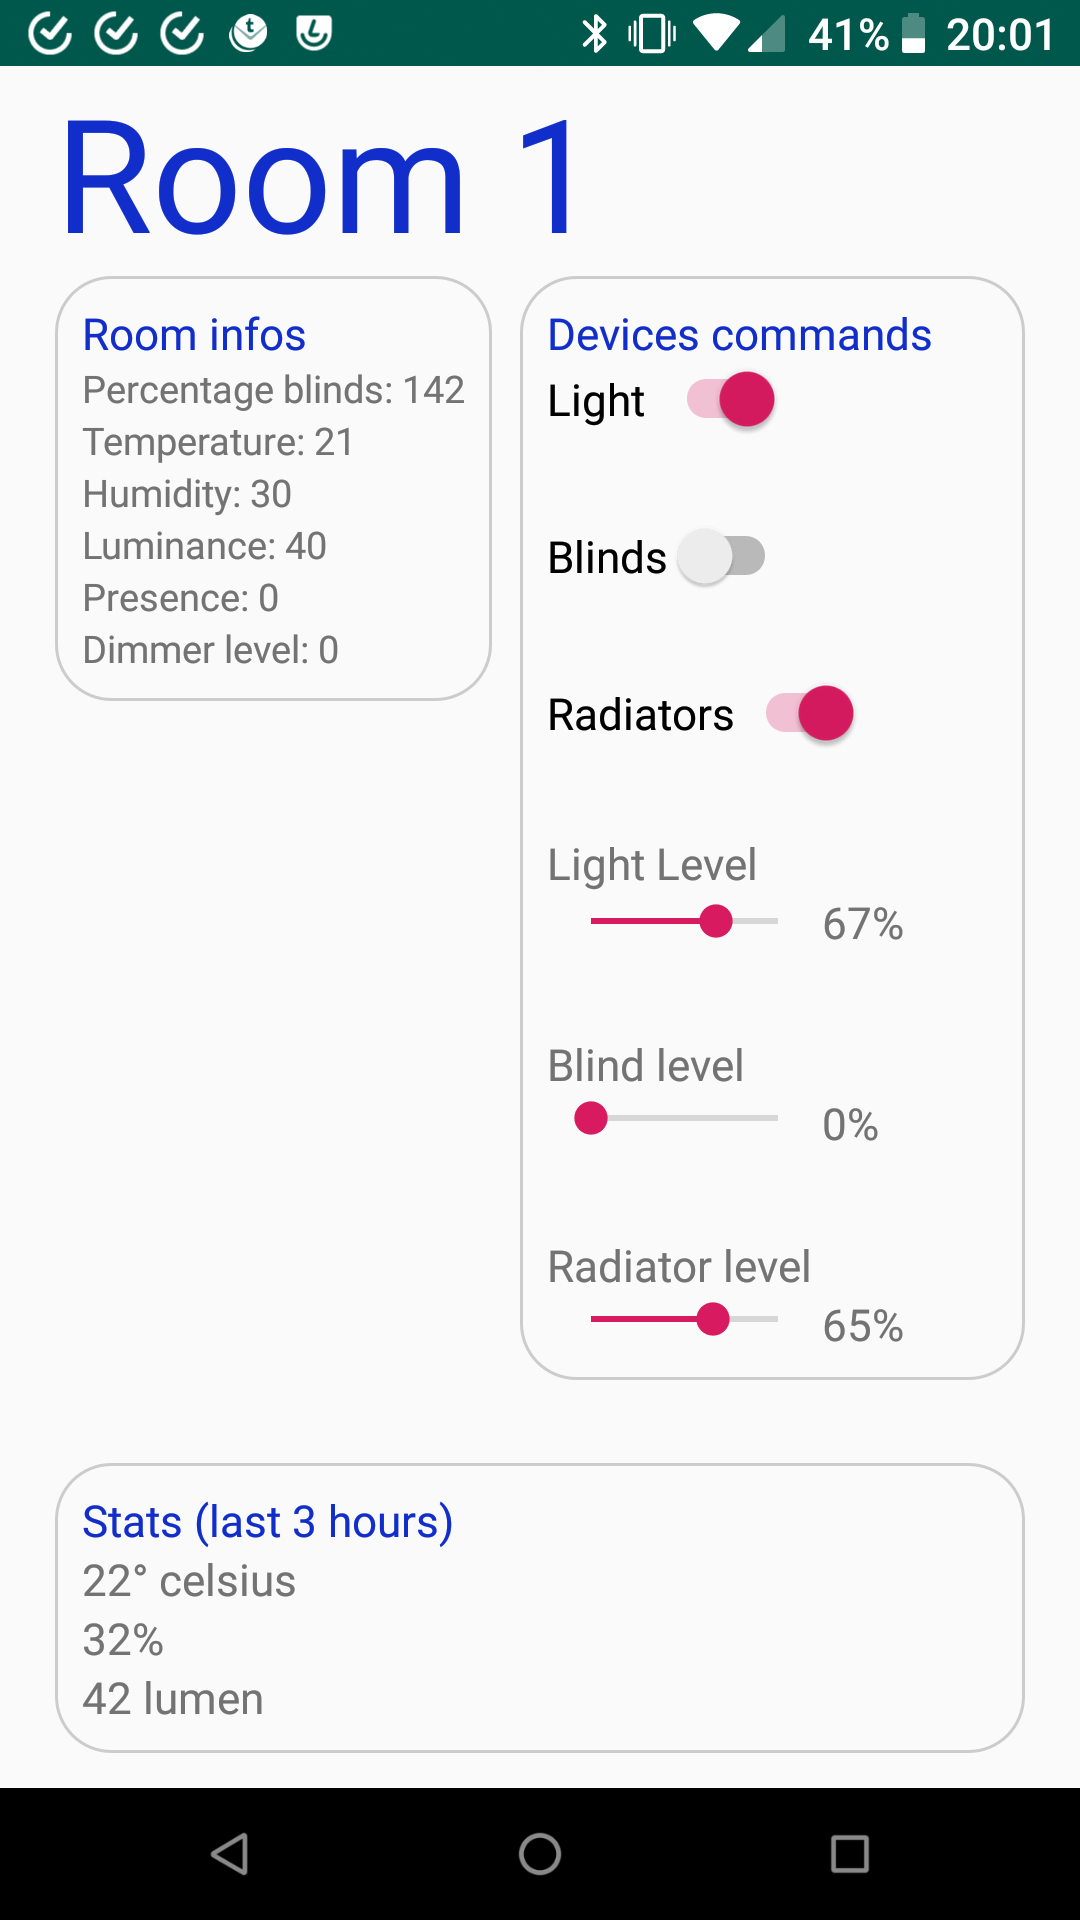
\includegraphics[width=0.35\textwidth]{img/app.png}
    \end{center}
    \caption{Application Android}
    \label{app_android}
\end{figure}

\subsection{Broker Kafka}
Le broker Kafka joue le rôle de coordinateur entre tous les différents clients qui consomment et produisent des messages dans les différents topics. Nous avons choisi de déployer ce broker Kafka sur une instance AWS \cite{aws} avec Docker \cite{docker} et docker-compose \cite{docker-compose}, le rendant accessible par toutes les entités du système.
Nous avons également associé un nom de domaine à cette instance, ce qui permet de la référencer de manière plus lisible et agréable par les clients. Nous avons fait usage des images docker de Confluent \cite{confluent} pour Kafka \cite{cp-kafka} et son Zookeeper \cite{cp-zookeeper}. Elles intègrent un broker Kafka configurable. Le listing \ref{compose-kafka} montre un exemple d'utilisation de ces images dans un \mintinline{text}{docker-compose.yml}. Dans cet exemple, le broker Kafka utilisé est disponible avec l'\acrshort{uri} \mintinline{text}{iot.liatti.ch} sur le port 29092.
\begin{code}
    \begin{minted}[bgcolor=mygray,breaklines,breaksymbol=,linenos,frame=single,stepnumber=1,tabsize=2]{yaml}
version: '3'
services:
  zookeeper:
    image: confluentinc/cp-zookeeper:latest
    environment:
      ZOOKEEPER_CLIENT_PORT: 2181
      ZOOKEEPER_TICK_TIME: 2000
  kafka:
    image: confluentinc/cp-kafka:latest
    depends_on:
      - zookeeper
    ports:
      - 29092:29092
    environment:
      KAFKA_BROKER_ID: 1
      KAFKA_ZOOKEEPER_CONNECT: zookeeper:2181
      KAFKA_ADVERTISED_LISTENERS: PLAINTEXT://kafka:9092,PLAINTEXT_HOST://iot.liatti.ch:29092
      KAFKA_LISTENER_SECURITY_PROTOCOL_MAP: PLAINTEXT:PLAINTEXT,PLAINTEXT_HOST:PLAINTEXT
      KAFKA_INTER_BROKER_LISTENER_NAME: PLAINTEXT
      KAFKA_OFFSETS_TOPIC_REPLICATION_FACTOR: 1
    \end{minted}
    \caption{Utilisation des images Docker de Confluent pour Kafka}
    \label{compose-kafka}
\end{code}

\subsection{\acrshort{rest} server Flask}
Etant donné qu'il n'existe pas encore de librairie permettant d'utiliser directement le client Kafka sur Android, nous avons du mettre en place un adapteur entre Kafka et Android.
Pour ce faire, nous avons utilisé la librairie Flask \cite{flask} de Python 3 qui permet de mettre en place une \acrshort{api} \acrshort{rest}. Ce serveur est connecté à la base de données et au broker Kafka. Le producteur Kafka se charge de transformer les actions reçues sous forme de requêtes HTTP en messages Kafka envoyés directement dans le bon topic, ce qui permet d'effectuer les actions demandées en conséquence (ouverture des stores par exemple). Pour récupérer l'état actuel des \textit{\textit{devices}} ou de la pièce, les derniers logs sont récupérés avec des requêtes à la base de données. Le serveur est déployé dans un container Docker avec docker-compose.

\subsubsection{Routes exposées}
Voici la liste exhaustive des différentes routes mise à disposition par notre \acrshort{api} \acrshort{rest} : 

\paragraph{KNX}

\begin{itemize}
  \item \mintinline{python}{Endpoint: "/open_blinds" -  Method: GET}
  \begin{itemize} 
    \item Params :
    \begin{itemize}
      \item uuid: string
      \item major: int
      \item minor: int
    \end{itemize}

    \item Response : 
    \begin{itemize}
      \item OK: \mintinline{json}{{ "success": true }}
      \item Error: \mintinline{json}{{ "success": false }}
    \end{itemize}
  \end{itemize}
\end{itemize}


\begin{itemize}
  \item \mintinline{python}{Endpoint: "/close_blinds" -  Method: GET}
  \begin{itemize} 
    \item Params :
    \begin{itemize}
      \item uuid: string
      \item major: int
      \item minor: int
    \end{itemize}

    \item Response : 
    \begin{itemize}
      \item OK: \mintinline{json}{{ "success": true }}
      \item Error: \mintinline{json}{{ "success": false }}
    \end{itemize}
  \end{itemize}
\end{itemize}

\begin{itemize}
  \item \mintinline{python}{Endpoint: "/percentage_blinds" -  Method: GET}
  \begin{itemize} 
    \item Params :
    \begin{itemize}
      \item uuid: string
      \item major: int
      \item minor: int
      \item percentage: int
    \end{itemize}

    \item Response : 
    \begin{itemize}
      \item OK: \mintinline{json}{{ "success": true }}
      \item Error: \mintinline{json}{{ "success": false }}
    \end{itemize}
  \end{itemize}
\end{itemize}

\begin{itemize}
  \item \mintinline{python}{Endpoint: "/percentage_radiator" -  Method: GET}
  \begin{itemize} 
    \item Params :
    \begin{itemize}
      \item uuid: string
      \item major: int
      \item minor: int
      \item percentage: int
    \end{itemize}

    \item Response : 
    \begin{itemize}
      \item OK: \mintinline{json}{{ "success": true }}
      \item Error: \mintinline{json}{{ "success": false }}
    \end{itemize}
  \end{itemize}
\end{itemize}


\paragraph{Infos}

\begin{itemize}
  \item \mintinline{python}{Endpoint: "/read_percentage_blinds" -  Method: GET}
  \begin{itemize} 
    \item Params :
    \begin{itemize}
      \item uuid: string
      \item major: int
      \item minor: int
    \end{itemize}

    \item Response : 
    \begin{itemize}
      \item OK: \mintinline{json}{{ "success": true, "percentage": 42 }}
      \item Error: \mintinline{json}{{ "success": false }}
    \end{itemize}
  \end{itemize}
\end{itemize}



\paragraph{OpenZWave}

\begin{itemize}
  \item \mintinline{python}{Endpoint: "/percentage_dimmers" -  Method: GET}
  \begin{itemize} 
    \item Params :
    \begin{itemize}
      \item uuid: string
      \item major: int
      \item minor: int
      \item percentage: int
    \end{itemize}

    \item Response : 
    \begin{itemize}
      \item OK: \mintinline{json}{{ "success": true }}
      \item Error: \mintinline{json}{{ "success": false }}
    \end{itemize}
  \end{itemize}
\end{itemize}

\paragraph{Infos}

\begin{itemize}
  \item \mintinline{python}{Endpoint: "/sensor_get_temperature" -  Method: GET}
  \begin{itemize} 
    \item Params :
    \begin{itemize}
      \item uuid: string
      \item major: int
      \item minor: int
    \end{itemize}

    \item Response : 
    \begin{itemize}
      \item OK: \mintinline{json}{{ "success": true, "value": 23 }}
      \item Error: \mintinline{json}{{ "success": false }}
    \end{itemize}
  \end{itemize}
\end{itemize}

\begin{itemize}
  \item \mintinline{python}{Endpoint: "/sensor_get_humidity" -  Method: GET}
  \begin{itemize} 
    \item Params :
    \begin{itemize}
      \item uuid: string
      \item major: int
      \item minor: int
    \end{itemize}

    \item Response : 
    \begin{itemize}
      \item OK: \mintinline{json}{{ "success": true, "value": 23 }}
      \item Error: \mintinline{json}{{ "success": false }}
    \end{itemize}
  \end{itemize}
\end{itemize}

\begin{itemize}
  \item \mintinline{python}{Endpoint: "/sensor_get_luminance" -  Method: GET}
  \begin{itemize} 
    \item Params :
    \begin{itemize}
      \item uuid: string
      \item major: int
      \item minor: int
    \end{itemize}

    \item Response : 
    \begin{itemize}
      \item OK: \mintinline{json}{{ "success": true, "value": 23 }}
      \item Error: \mintinline{json}{{ "success": false }}
    \end{itemize}
  \end{itemize}
\end{itemize}

\begin{itemize}
  \item \mintinline{python}{Endpoint: "/sensor_get_motion" -  Method: GET}
  \begin{itemize} 
    \item Params :
    \begin{itemize}
      \item uuid: string
      \item major: int
      \item minor: int
    \end{itemize}

    \item Response : 
    \begin{itemize}
      \item OK: \mintinline{json}{{ "success": true, "value": 23 }}
      \item Error: \mintinline{json}{{ "success": false }}
    \end{itemize}
  \end{itemize}
\end{itemize}

\begin{itemize}
  \item \mintinline{python}{Endpoint: "/dimmer_get_level" -  Method: GET}
  \begin{itemize} 
    \item Params :
    \begin{itemize}
      \item uuid: string
      \item major: int
      \item minor: int
    \end{itemize}

    \item Response : 
    \begin{itemize}
      \item OK: \mintinline{json}{{ "success": true, "value": 23 }}
      \item Error: \mintinline{json}{{ "success": false }}
    \end{itemize}
  \end{itemize}
\end{itemize}

\paragraph{Autres routes}

\begin{itemize}
  \item \mintinline{python}{Endpoint: "/get_beacons" -  Method: GET}
  \begin{itemize}
    \item Response : 
    \begin{itemize}
      \item OK: \mintinline{json}{{ "success": true, "beacons": 23 }}
      \item Error: \mintinline{json}{{ "success": false }}
    \end{itemize}
  \end{itemize}
\end{itemize}

\begin{itemize}
  \item \mintinline{python}{Endpoint: "/get_devices" -  Method: GET}
  \begin{itemize} 
    \item Params :
    \begin{itemize}
      \item uuid: string
      \item major: int
      \item minor: int
    \end{itemize}

    \item Response : 
    \begin{itemize}
      \item OK: \mintinline{json}{{ "success": true, "devices": 23 }}
      \item Error: \mintinline{json}{{ "success": false }}
    \end{itemize}
  \end{itemize}
\end{itemize}

\paragraph{Stats}

\begin{itemize}
  \item \mintinline{python}{Endpoint: "/avg_temperature" -  Method: GET}
  \begin{itemize} 
    \item Params :
    \begin{itemize}
      \item uuid: string
      \item major: int
      \item minor: int
    \end{itemize}

    \item Response : 
    \begin{itemize}
      \item OK: \mintinline{json}{{ "success": true, "avg_temperature": 23 }}
      \item Error: \mintinline{json}{{ "success": false }}
    \end{itemize}
  \end{itemize}
\end{itemize}

\begin{itemize}
  \item \mintinline{python}{Endpoint: "/avg_humidity" -  Method: GET}
  \begin{itemize} 
    \item Params :
    \begin{itemize}
      \item uuid: string
      \item major: int
      \item minor: int
    \end{itemize}

    \item Response : 
    \begin{itemize}
      \item OK: \mintinline{json}{{ "success": true, "avg_humidity": 23 }}
      \item Error: \mintinline{json}{{ "success": false }}
    \end{itemize}
  \end{itemize}
\end{itemize}

\begin{itemize}
  \item \mintinline{python}{Endpoint: "/avg_luminance" -  Method: GET}
  \begin{itemize} 
    \item Params :
    \begin{itemize}
      \item uuid: string
      \item major: int
      \item minor: int
    \end{itemize}

    \item Response : 
    \begin{itemize}
      \item OK: \mintinline{json}{{ "success": true, "avg_luminance": 23 }}
      \item Error: \mintinline{json}{{ "success": false }}
    \end{itemize}
  \end{itemize}
\end{itemize}




\subsection{Modules KNX et Openzwave}
En se basant sur le code des exercices KNX et Openzwave réalisés en cours, nous avons créé deux modules reliant d'une part Kafka et KNX et d'autre part Kafka et Openzwave. Ces deux modules ont un fonctionnement similaire, ils sont constitués d'une librairie reprenant les méthodes pour communiquer avec KNX ou Openzwave et exposant les différentes méthodes relatives à l'utilisation des \textit{\textit{devices}}. Ils sont également constitués d'un fichier principal (\mintinline{text}{knx.py} et \mintinline{text}{zwave.py}), chaque fichier démarre un thread producteur Kafka, envoyant à intervalles réguliers les valeurs des stores, des senseurs et \textit{dimmers} Openzwave, et un thread consommateur Kafka, écoutant sur le topic "knx" ou "zwave" les commandes à effectuer sur les \textit{\textit{devices}}.

\subsection{Protocole des messages}
En ce qui concerne les messages consommés par KNX et Openzwave, nous avons choisi de définir notre propre protocole.
Celui-ci fait correspondre la clé du message reçu à l'action à effectuer et le contenu du message aux éventuels paramètres à transmettre. Ces différents paramètres sont au format \acrshort{json} puis encodés en bytes afin d'être transmis au broker Kafka et consommés par une autre entité.

\subsubsection{KNX}
Pour KNX nous retrouvons les messages suivants : 
\paragraph{Production}
\begin{itemize}
    \item \mintinline{text}{read_percentage_blinds} : Ce messages est produit à intervalles de 5 secondes, il permet d'envoyer dans le topic \mintinline{text}{knx} le pourcentage d'ouverture de tous les stores de toutes les salles. 
\end{itemize}

\paragraph{Consommation}
L'étage et la chambre permettent d'identifier l'appareil sur lequel il faut agir, pour cela ces deux paramètres sont donnés dans le corps du message ce qui permet d'intéragir avec le bon \textit{device} en fonction de la position de l'utilisateur.
\begin{itemize}
    \item \mintinline{text}{open_blinds} : permet d'ouvrir les stores (100\%)
    \item \mintinline{text}{close_blinds} : permet de fermer les stores (0\%)
    \item \mintinline{text}{percentage_blinds} : met les stores à un certain pourcentage qui est passé dans la valeur du message
    \item \mintinline{text}{percentage_radiator} : met les radiateurs à un certain pourcentage qui est passé dans la valeur du message
\end{itemize}

\subsubsection{Openzwave}
Openzwave est capable de traiter les messages suivants : 
\paragraph{Production}
\begin{itemize}
    \item \mintinline{text}{sensors_get_temperature} : produit la valeur de température de chaque senseur
    \item \mintinline{text}{sensors_get_humidity} : produit la valeur de l'humidité de chaque senseur
    \item \mintinline{text}{sensors_get_luminance} : produit la valeur de la luminance de chaque senseur
    \item \mintinline{text}{sensors_get_motion} : produit une indication de présence de chaque senseur
    \item \mintinline{text}{dimmers_get_level} : produit la valeur de chaque variateur (\textit{dimmer})
\end{itemize}

\paragraph{Consommation}
\begin{itemize}
    \item \mintinline{text}{dimmers_set_level} : met les \textit{dimmers} à un certain pourcentage
\end{itemize}

\subsection{Base de données}
En ce qui concerne la base de données, nous avons opté pour une base relationnelle avec MySQL \cite{mysql} qui nous a permis de représenter les différentes entités et les lier facilement et de manière efficace. Comme représenté sur la figure \ref{db_schema}, la base comporte six tables :
\begin{itemize}
    \item \mintinline{text}{Beacon} : contient tous les Beacons et dans quelle pièce
    \item \mintinline{text}{Room} : contient les différentes pièces et à quel étage
    \item \mintinline{text}{Device} : contient tous les \textit{devices} (KNX et Openzwave), identifiés de manière unique et dans quelle pièce ils se trouvent
    \item \mintinline{text}{KnxNode} : contient les informations concernant les \textit{devices} KNX uniquement (type, bloc et étage)
    \item \mintinline{text}{ZwaveNode} : contient les informations concernant les \textit{devices} Openzwave uniquement (identifiant dans le réseau Openzwave et nom)
    \item \mintinline{text}{Log} : contient les logs produits par tous les \textit{devices} avec la valeur, le type de valeur et le \textit{timestamp} (à la seconde) de la mesure
\end{itemize}
Ces relations permettent des usages tels que :
\begin{itemize}
    \item Pour un Beacon donné, retrouver tous les logs des \textit{devices} de la pièce associée
    \item Avec un type, bloc et étage KNX donnés, retrouver dans quelle pièce ils se trouvent
    \item Réaliser des statistiques sur les logs, comme la température moyenne dans une pièce
\end{itemize}

Voici le diagramme représentant notre base de données :
\begin{figure}
    \begin{center}
        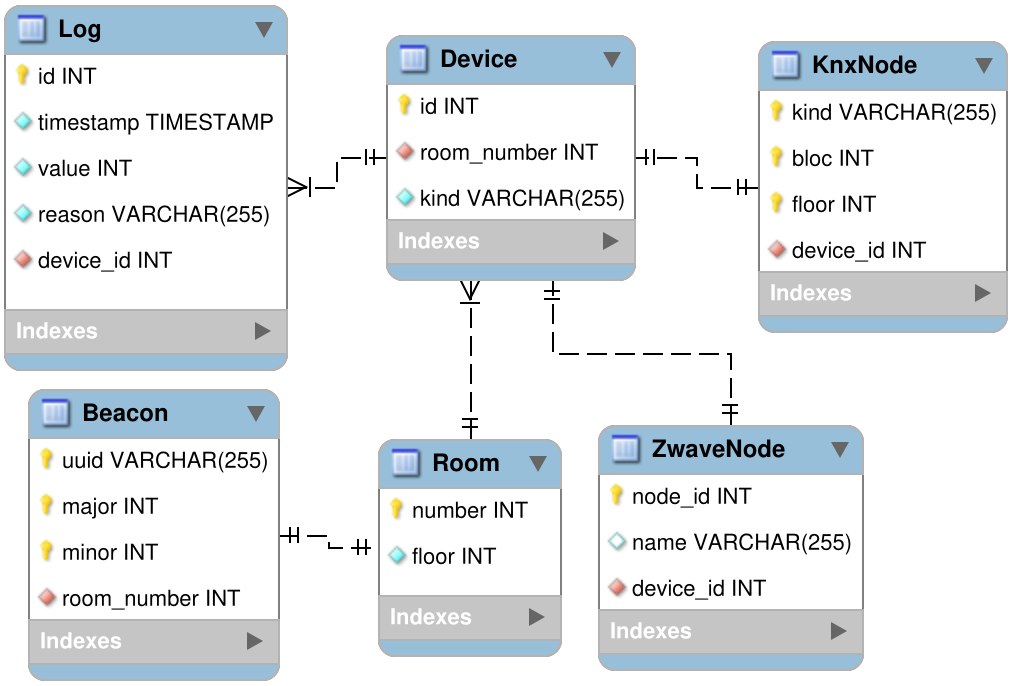
\includegraphics[width=0.8\textwidth]{img/mysql-shema.png}
    \end{center}
    \caption{Schéma relationnel de la base de données}
    \label{db_schema}
\end{figure}

\subsection{Automatic controller}
Le contrôleur automatique est déployé dans un container Docker avec docker-compose. Son rôle est de gérer les états des \textit{devices} dans les différentes salles. Pour ce faire, il lit les messages dans les topics Kafka propres à KNX et Openzwave. En fonction des informations récupérées sur les \textit{devices}, il applique certaines règles logiques afin de contrôler les \textit{devices} automatiquement.
Les différentes règles sont les suivantes (à savoir que les différentes valeurs définies sont arbitraires et modifiables très facilement) :
\begin{itemize}
  \item Si aucune présence est détectée dans la pièce, le radiateur se met automatiquement à 10\% afin d'économiser de l'énergie
  \item Si quelqu'un est dans la pièce, le radiateur se règle à 90\% afin que la personne n'ait pas froid
  \item Si l'humidité est supérieure à 50\% les stores de la pièce se ferment
  \item S'il est plus tôt que 19 heures, que quelqu'un est présent dans la pièce et que la luminosité est faible, les stores s'ouvrent automatiquement
  \item Si l'heure actuelle est comprise entre 19 heures et 7 heures du matin et que quelqu'un est présent dans la pièce, ou, si la luminosité est trop faible, la lumière s'allume alors automatiquement. Dans un des cas contraires, la lumière s'éteint.
\end{itemize}

\subsection{DB to Kafka}
Pour minimiser les dépendances à la base de données pour les modules KNX, OpenZWave et Automatic controller, nous avons réalisé un connecteur, \mintinline{python}{db_to_kafka.py}, qui produit dans le topic Kafka \mintinline{text}{db} la liste de tous les \textit{devices} avec leur type effectif (KNX ou OpenZWave) et leur emplacement physique (dans quelle pièce ils se trouvent). Ainsi, les modules reliés à Kafka nécessitant les informations sur les \textit{devices} peuvent relire le topic \mintinline{text}{db} à partir de l'\textit{offset} zéro pour obtenir tous les \textit{devices}. Ce module est déployé dans un container Docker avec docker-compose.

\subsection{Logs et statistiques}
Pour garder une trace des valeurs des différents \textit{devices}, un module \mintinline{python}{logs.py} écoute et consomme les messages Kafka des topics \mintinline{text}{knx} et \mintinline{text}{zwave} concernant la lecture des valeurs et réalise des insertions en base de données dans la table \mintinline{text}{Log}. Il est donc aisé de retrouver les anciennes valeurs des capteurs et réaliser des statistiques avec. Ce module est déployé dans un container Docker avec docker-compose.

\newpage

\section{Conclusion} %-----------------------------------------------------------------------------------------------
\subsection{Bilan personnel}
Pour conclure, ce projet nous a permit d'apprendre et pratiquer Kafka, une technologie initaliemment inconnue, ce qui fût très instructif. Il nous à également permis d'approfondir les notions vue en cours concernant KNX, Openzwave et la detection des beacons depuis un appareil Android. En ajoutant a tout cela une partie devloppement Android, une base de données SQL et l'utilisation de python. Ce qui fait de ce projet un très bon cas pratique permettant de mettre en lien toutes ces technologies plus interessante les unes que les autres.
% TODO: Sucage de boule

\subsection{Problèmes rencontrés}
Les principales difficultés rencontrées durant le développement de ce projet sont les suivantes :
\begin{itemize}
    \item Docker python
    \item KNX la documentation fournie ne correspondait pas parfaitement avec le fonctionnement réeé du protocole
    \item Openzwave manque d'informations concernant le reset manuel du controller
\end{itemize}

% TODO: améliorations
\subsection{Améliorations possibles}
Les améliorations suivantes pourraient être apportées au projet :
\begin{itemize}
    \item
\end{itemize}
\newpage

\section{Références} %-----------------------------------------------------------------------------------------------
\bibliographystyle{unsrt}
\bibliography{bib}

\end{document}

% \begin{figure}
%     \begin{center}
%         \includegraphics[width=0.8\textwidth]{images/image.png}
%     \end{center}
%     \caption{légende}
%     \label{label}
% \end{figure}

% \bigbreak
% \begin{code}
%     \begin{minted}[bgcolor=mygray,breaklines,breaksymbol=,linenos,frame=single,stepnumber=1,tabsize=2]{rust}
% fn main() {
%     println!("Hello, world!");
% }
%     \end{minted}
%     \caption{Hello world en Rust}
%     \label{label}
% \end{code}
% \bigbreak

% \bigbreak
% \begin{code}
%     \inputminted[bgcolor=mygray,breaklines,breaksymbol=,linenos,frame=single,stepnumber=1,
%         tabsize=2,firstline=157,lastline=185]{rust}{file.rs}
%     \caption{légende}
%     \label{label}
% \end{code}
% \bigbreak
